% =====================================================================
% clasificacion.tex
% Responsabilidad única: presentar el análisis de clasificación del riesgo
% de no conformidad (modelos del curso, Taguchi, sobremuestreo,
% calibración y umbral por costo con alertas por semana).
% Cifras: macros Clf*; tablas tabla_clf_*; figuras 05_*.
% =====================================================================
\section{Clasificación: Riesgo de no conformidad}
\label{sec:clasificacion}

La segunda pregunta sigue los mismos tres niveles de la regresión, pero aquí
aparecen dos problemas que allá no estaban. Hay pocas no conformes y eso
obliga a pensar en el sobremuestreo. Además la salida tiene que ser una
probabilidad que se pueda creer porque de ella dependen el umbral de alerta
y la capa bayesiana de la Sección~\ref{sec:bayes}.

El análisis \codigo{\ClfAnalisis} estima en el momento \codigo{\ClfMomento}
la probabilidad de que una muestra aceptada resulte no conforme
(\codigo{\ClfObjetivo}), con lo que se sabe al recibirla: El cliente y su
historial reciente, el producto y su matriz, el ensayo, las condiciones de
transporte y el calendario. En entrenamiento hay
\ClfMuestrasEntrenamiento{} muestras con \ClfPositivosEntrenamiento{} no
conformes (\ClfPrevalenciaEntrenamientoPct{}\,\%) y en validación
\ClfMuestrasValidacion{} con \ClfPositivosValidacion{}
(\ClfPrevalenciaValidacionPct{}\,\%).

\subsection{Pasada didáctica con los modelos del curso}

En la pasada didáctica (Tabla~\ref{tab:clf-didactica}) el mejor modelo fue la
\MakeLowercase{\ClfMejorDidactico}, con un ROC-AUC medio de
\ClfAUCMejorDidactico{} y una desviación de \ClfAUCDesvMejorDidactico{} entre
bloques. Su precisión media fue de \ClfPrecisionMediaMejorDidactico{} frente a
\ClfDummyPrecisionMedia{} del clasificador que solo predice la proporción de
no conformes, o sea que el modelo sí encuentra no conformes bastante por
encima de lo que daría el azar. El perceptrón multicapa quedó cerca
(\ClfAUCMLPDidactico{}) y el más débil fue \ClfPeorDidactico{}
(\ClfAUCPeorDidactico{}). Una explicación posible es que con decenas de
columnas codificadas todas las muestras quedan casi igual de lejos entre sí y
la distancia deja de distinguir a los vecinos.

\begin{table}[!htbp]
\centering
\tablaancha{clf_didactica}
\caption{Pasada didáctica de clasificación con la media y la desviación entre
bloques temporales: La habilidad es $2\,\mathrm{AUC}-1$ y la regresión
logística tiene el mayor ROC-AUC medio.}
\label{tab:clf-didactica}
\end{table}

El árbol sin poda crece hasta \ClfHojasSinPoda{} hojas y obtiene un ROC-AUC de
\ClfAUCSinPoda{}, mientras que la poda con $\alpha=\ClfAlfaPoda$ lo deja en
\ClfHojasPodado{} hojas con \ClfAUCPodado{}, es decir que quedó más simple y
mejor. Su hoja de mayor riesgo reúne \ClfHojaRiesgoFilas{} muestras con una
fracción de no conformes de \ClfHojaRiesgoFraccion{}, unas
\ClfHojaRiesgoVeces{} veces la tasa general. Las reglas de sus hojas más
riesgosas combinan el historial de no conformidad del producto con la
temperatura por las horas de transporte, que es la misma interacción que vimos
en la Figura~\ref{fig:transporte}.

En la regresión logística la variable que más sube el riesgo es
\codigo{\ClfVariableSube}, con una razón de odds de \ClfOddsSube{} (con las
demás variables fijas, sus odds de salir no conforme son unas
\ClfOddsSube{} veces las del resto) y la que más lo baja es
\codigo{\ClfVariableBaja} (\ClfOddsBaja{}). Estas razones solo valen para los
datos simulados porque esas relaciones las fijó el generador.

\paragraph{Efecto del sobremuestreo.} Sospechábamos que el sobremuestreo no le
pega igual a todos los modelos así que repetimos cada modelo de la pasada
con sobremuestreo de la clase minoritaria dentro de la tubería, sin tocar los
pliegues de validación (Tabla~\ref{tab:clf-sobre}). A la
\MakeLowercase{\ClfSobreMenosPierde} casi no le cambia el ROC-AUC
(\ClfSobreDeltaAUCMenor{}), pero al \MakeLowercase{\ClfSobreMasPierde} le
quita \ClfSobreDeltaAUC{}, algo que retomamos en la
Sección~\ref{sec:redes}. Lo más importante es que en todos los modelos el
puntaje de Brier empeora y la probabilidad media predicha se dispara. Es la
descalibración que esperábamos: El modelo aprende con una proporción de no
conformes que no es la real y aunque el orden de las muestras cambie poco sus
cifras dejan de ser probabilidades así que no podrían alimentar la capa
bayesiana sin recalibrarse.

\begin{table}[!htbp]
\centering
\tablacompacta{clf_sobremuestreo}
\caption{Modelos didácticos sin y con sobremuestreo: El ROC-AUC cambia poco
salvo en el perceptrón, pero el Brier y la probabilidad media muestran que el
sobremuestreo descalibra las probabilidades de todos.}
\label{tab:clf-sobre}
\end{table}

\subsection{Taguchi y búsqueda en rejilla}

En el L16 de clasificación el factor más influyente vuelve a ser el
\ClfFactorPrincipal{} (delta de \ClfDeltaPrincipal{} dB), seguido del
\ClfFactorSegundo{} (\ClfDeltaSegundo{} dB) y el escalado vuelve a ser
indiferente. El óptimo aditivo es \emph{\ClfOptimo}, con una S/N predicha de
\ClfSNPredicha{} dB (que equivale a un ROC-AUC de
\ClfAUCEquivalentePredicha{}). En la confirmación observamos \ClfSNObservada{}
dB (ROC-AUC de \ClfAUCConfirmacion{}), dentro de la tolerancia de
\ClfToleranciaSN{} dB. Como la confirmación superó a la mejor corrida
observada (la \ClfMejorCorrida{}, con \ClfSNMejorCorrida{} dB y ROC-AUC de
\ClfAUCMejorCorrida{}), a la rejilla pasó la configuración de la
\ClfOrigenConfiguracion{}.

Ese óptimo incluye el sobremuestreo, que en el promedio del L16 sube un poco
la S/N aunque en la logística de la pasada casi no movió el ROC-AUC. Como ya
sabíamos que descalibra lo dejamos con la condición de calibrar después. En la rejilla la logística
(\ClfRejillaLogisticaAUC{}) quedó por delante del árbol
(\ClfRejillaArbolAUC{}) con \ClfHiperparametros{} y un ROC-AUC por bloque de
\ClfAUCRejillaFinal{}, sin necesidad de la regla de empate
(\ClfPorEmpate{}).

\subsection{Validación y calibración}

En validación la logística ordenó mejor que el árbol, con un ROC-AUC de
\ClfAUCValidacionSinCalibrar{} antes de calibrar frente a
\ClfAUCValidacionOtro{} del \MakeLowercase{\ClfModeloOtro}. Sin embargo su
Brier sin calibrar (\ClfBrierSinCalibrar{}) es peor que el del clasificador
constante (\ClfDummyBrier{}), lo que confirma la descalibración que mete el
sobremuestreo. Por eso le ajustamos una calibración sigmoide con los bloques
temporales de entrenamiento, que es una curva en forma de S que convierte el
puntaje del modelo en una probabilidad que se parece a la frecuencia real.
Con ella el Brier baja a \ClfBrierCalibrado{} y la probabilidad media pasa
de \ClfProbMediaSinCalibrar{} a \ClfProbMediaCalibrado{}, cerca de la tasa
real, mientras que el orden casi no cambia. El ROC-AUC calibrado es de
\ClfAUCCalibrado{} (IC 95\,\% de \ClfAUCValidacionInf{} a
\ClfAUCValidacionSup{}) y la precisión media de \ClfPrecisionMediaValidacion{}.

\begin{figure}[!htbp]
\centering
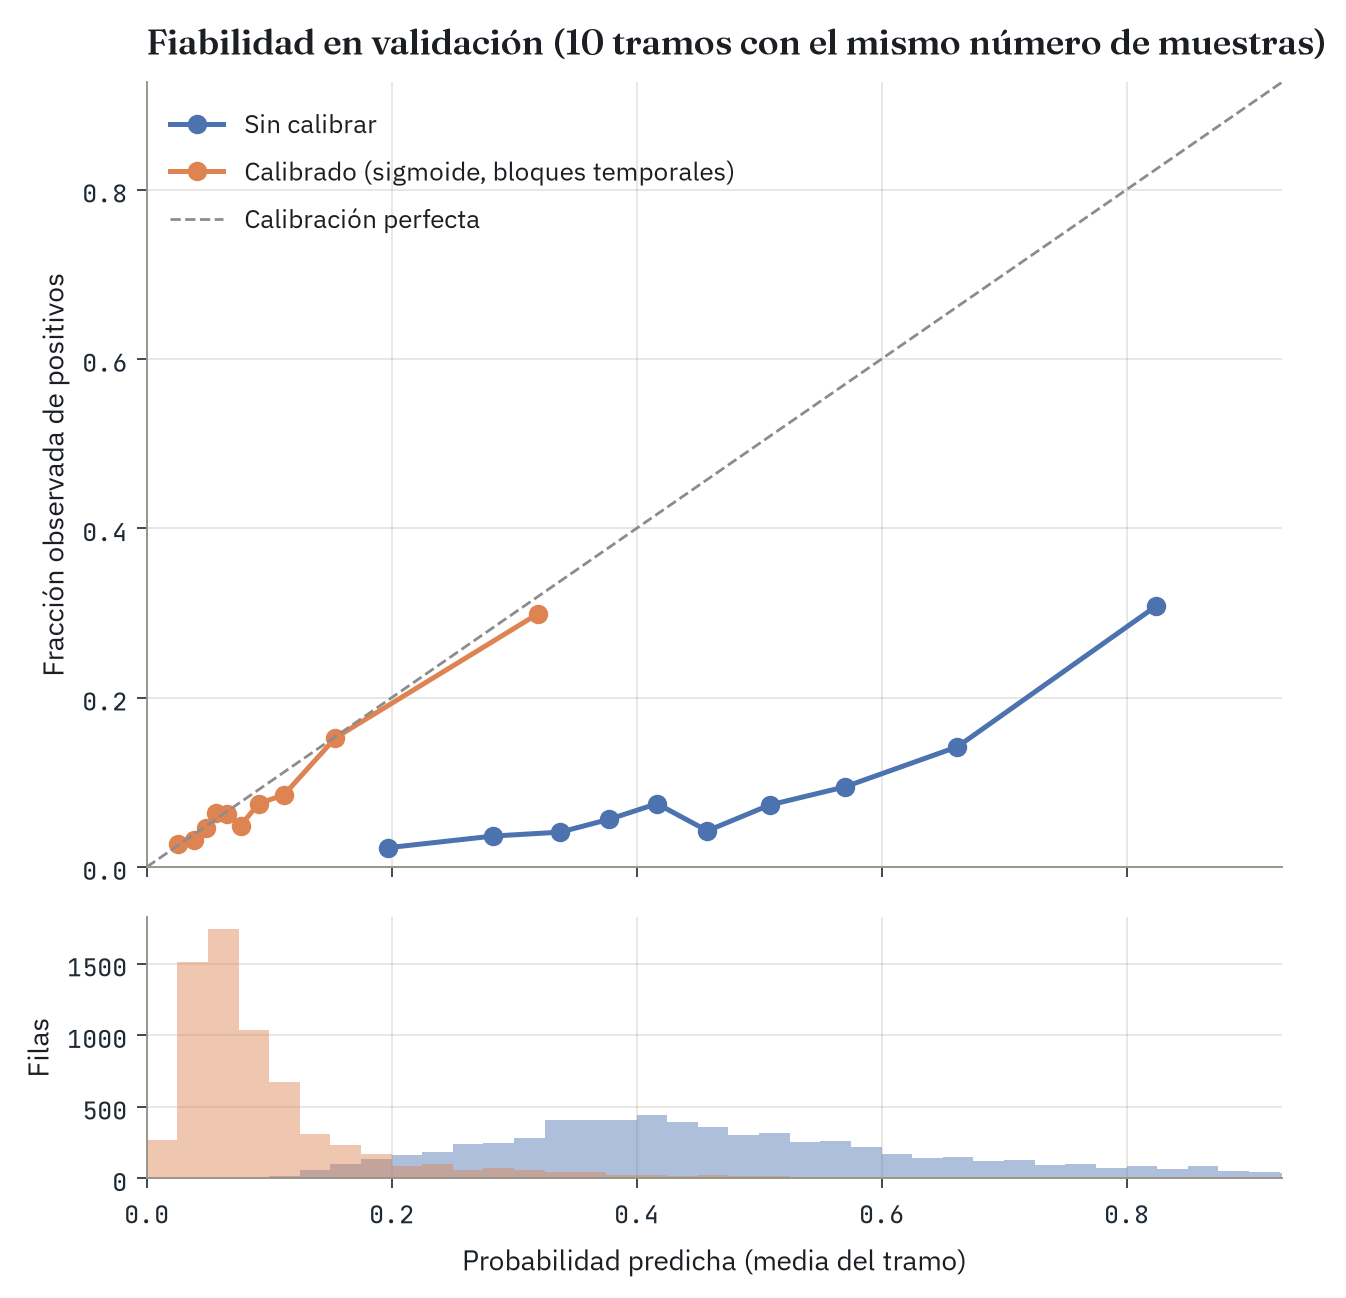
\includegraphics[width=0.46\textwidth]{04_fiabilidad.png}
\caption{Fiabilidad en validación, con tramos del mismo número de muestras:
Sin calibrar (azul) las probabilidades quedan muy por debajo de la diagonal y
muy por encima de la tasa real (\ClfPrevalenciaValidacionPct{}\,\%), mientras
que la calibración sigmoide (naranja) las devuelve a la diagonal y al rango
bajo, donde está casi toda la masa (histograma inferior).}
\label{fig:fiabilidad}
\end{figure}

\subsection{Umbral por costo y alertas por semana}

Con las probabilidades calibradas el umbral de menor costo en validación
coincide con el teórico, $t=\ClfUmbral$ (Figura~\ref{fig:umbrales}), lo que es
una señal de que la calibración funcionó. Con ese umbral se emiten
\ClfAlertasValidacion{} alertas en las \ClfSemanasValidacion{} semanas de
validación, unas \ClfAlertasSemana{} por semana, con $\text{TP}=\ClfTP$,
$\text{FP}=\ClfFP$, $\text{FN}=\ClfFN$ y $\text{TN}=\ClfTN$. Eso da una
precisión de \ClfPrecisionUmbral{}, un recall de \ClfRecallUmbral{} y un F1
de \ClfFUnoUmbral{}. El costo es de \ClfUmbralCosto{} (IC 95\,\% de
\ClfUmbralCostoInf{} a \ClfUmbralCostoSup{}) frente a \ClfCostoNoAlertar{} de
no alertar nunca y \ClfCostoAlertarTodo{} de alertar todas, un ahorro del
\ClfAhorroPct{}\,\% frente a la mejor política sin modelo.

\begin{figure}[!htbp]
\centering
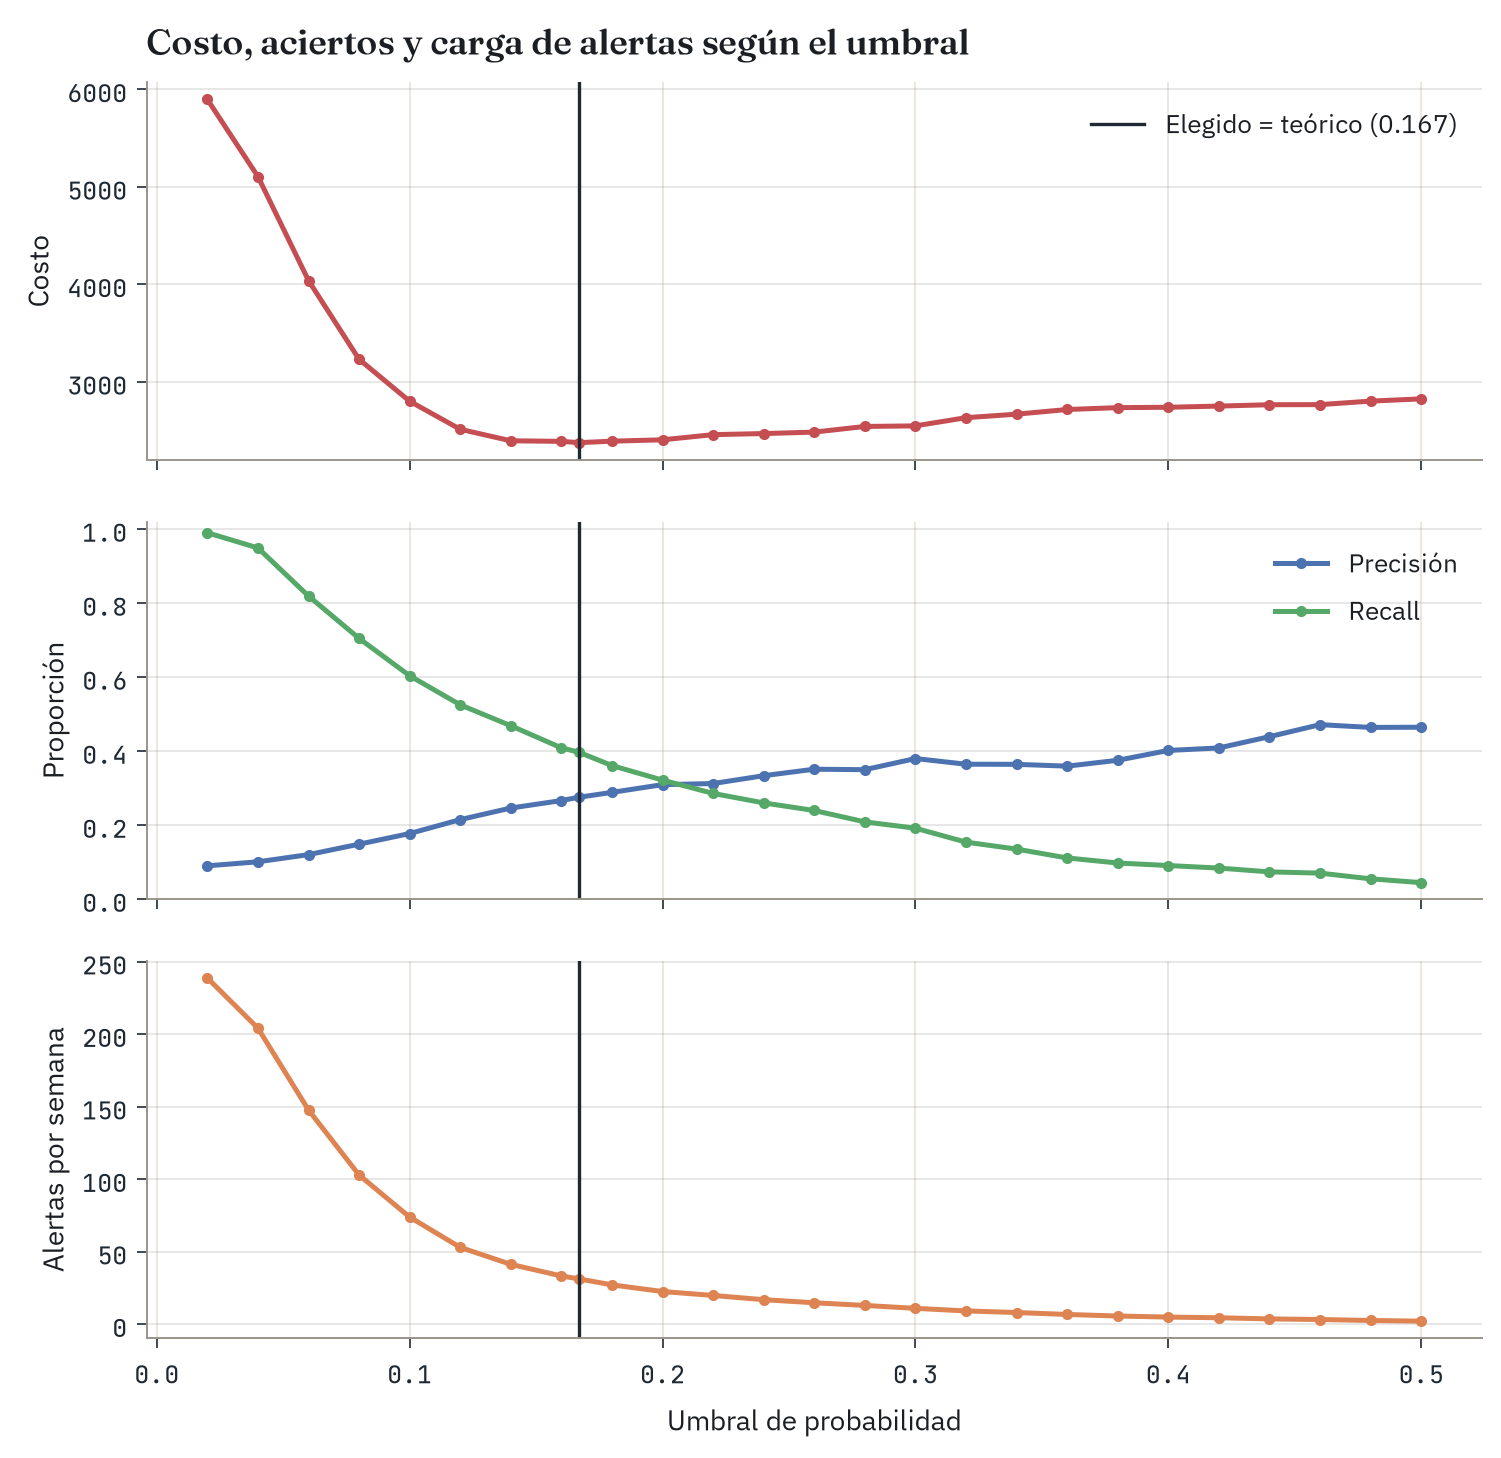
\includegraphics[width=0.48\textwidth]{04_umbrales.png}
\caption{Costo, precisión, recall y alertas por semana según el umbral en
validación, con el umbral elegido como línea vertical: El costo es casi plano
alrededor del umbral teórico mientras que las alertas por semana cambian
mucho a su izquierda.}
\label{fig:umbrales}
\end{figure}

Dicho en términos del laboratorio, por cada no conforme que la alerta detecta
se revisan unas \ClfRevisadasPorDetectado{} muestras que resultan conformes y
aun así se escapa más de la mitad de las no conformes (recall de
\ClfRecallUmbral{}). O sea que la alerta serviría para priorizar la revisión
y no para reemplazar el análisis de todas las muestras. Por último el modelo
congelado (\MakeLowercase{\ClfModeloFinal} calibrada con umbral
\ClfUmbral{}) lo reajustamos con entrenamiento más validación
(\ClfFilasReajuste{} muestras).
